%!TEX root = ../Thesis.tex
\section*{Anhang}
\addcontentsline{toc}{section}{Anhang}
\fancyhead[R]{Anhang}

\anhangsverzeichnis

\anhang{Listings}\label{app:Listing}

\begin{figure}[bht]
	\begin{lstlisting}[caption=Exemplarische Konfiguration Module Federation Portalshell, label=lst:ModuleFederationWebpackShell, language=Javascript]
		[...]
		plugins: [
		new ModuleFederationPlugin({
			
			remotes: {
				"microapp": "microapp@http://localhost:3000/remoteEntry.js",
			},
			shared: share({
				"@angular/core": { singleton: true, strictVersion: true, requiredVersion: 'auto' }, 
				"@angular/common": { singleton: true, strictVersion: true, requiredVersion: 'auto' }, 
				"@angular/common/http": { singleton: true, strictVersion: true, requiredVersion: 'auto' }, 
				"@angular/router": { singleton: true, strictVersion: true, requiredVersion: 'auto' },
				
				...sharedMappings.getDescriptors()
			})
			
		}),
		sharedMappings.getPlugin()
		],
		[...]
	\end{lstlisting}
	\footnoterule{}
	\footnotesize{Auszug aus der \texttt{webpack.config.js} einer Portalshell}
\end{figure}

\newpage
\begin{figure}[bht]
	\begin{lstlisting}[caption=Exemplarische Konfiguration Module Federation Microfrontend, label=lst:ModuleFederationWebpackRemote, language=Javascript]
		[...]
		plugins: [
		new ModuleFederationPlugin({      
			name: "microapp",
			filename: "remoteEntry.js",  
			exposes: {
				'./Module': './src/app/distant/distant.module.ts',
			},
			shared: share({
				"@angular/core": { singleton: true, strictVersion: true, requiredVersion: 'auto' }, 
				"@angular/common": { singleton: true, strictVersion: true, requiredVersion: 'auto' }, 
				"@angular/common/http": { singleton: true, strictVersion: true, requiredVersion: 'auto' }, 
				"@angular/router": { singleton: true, strictVersion: true, requiredVersion: 'auto' },
				
				...sharedMappings.getDescriptors()
			})        
		}),
		sharedMappings.getPlugin()
		],
		[...]
	\end{lstlisting}
	\footnoterule{}
	\footnotesize{Auszug aus der \texttt{webpack.config.js} eines Microfrontends}
\end{figure}

\newpage
\begin{figure}[bht]
	\begin{lstlisting}[caption=Konfiguration eines Module Federation Microfrontends, label=lst:WebpackConfigMF, language=Javascript]
		[...]
		plugins: [
		new ModuleFederationPlugin({
			library: { type: "module" },
			
			name: "evalmf",
			filename: "remoteEntry.js",
			exposes: {
				'./Module': './src/app/export/export.module.ts',
			},   
			
			shared: share({
				"@angular/core": { singleton: true, strictVersion: true, requiredVersion: 'auto' }, 
				"@angular/common": { singleton: true, strictVersion: true, requiredVersion: 'auto' }, 
				"@angular/common/http": { singleton: true, strictVersion: true,	requiredVersion: 'auto' }, 
				"@angular/router": { singleton: true, strictVersion: true, requiredVersion: 'auto' },
				"@angular/material": { singleton: true, strictVersion: true, requiredVersion: 'auto' },
				
				...sharedMappings.getDescriptors()
			})
			
		}),
		sharedMappings.getPlugin()
		],
		[...]
	\end{lstlisting}
	\footnoterule{}
	\footnotesize{Auszug aus der \texttt{webpack.config.js} eines Microfrontends}
\end{figure}

\newpage
\begin{figure}[bht]
	\begin{lstlisting}[caption=Konfiguration einer Module Federation Portalshell, label=lst:WebpackConfigPS, language=Javascript]	
		[...]
		plugins: [
		new ModuleFederationPlugin({
			library: { type: "module" },
			shared: share({
				"@angular/core": { singleton: true, strictVersion: true, requiredVersion: 'auto' }, 
				"@angular/common": { singleton: true, strictVersion: true, requiredVersion: 'auto' }, 
				"@angular/common/http": { singleton: true, strictVersion: true,	requiredVersion: 'auto' }, 
				"@angular/router": { singleton: true, strictVersion: true, requiredVersion: 'auto' },
				"@angular/material": { singleton: true, strictVersion: true, requiredVersion: 'auto' },
				
				...sharedMappings.getDescriptors()
			})
			
		}),
		sharedMappings.getPlugin()
		],
		[...]
	\end{lstlisting}
	\footnoterule{}
	\footnotesize{Auszug aus der \texttt{webpack.config.js} der Portalshell}
\end{figure}

\newpage
\begin{figure}[bht]
	\begin{lstlisting}[caption=Einbindung eines Module Federation Microfrontend, label=lst:MFPSConfig2, language=Javascript]
		// decl.d.ts
		declare module 'evalmf/Module';
		
		// app.routes.ts
		const URL = 'http://localhost:4202/remoteEntry.js';
		{
			path: 'EvalMF',
			loadChildren: () => loadRemoteModule({
				type: 'module',
				remoteEntry: URL,
				exposedModule: './Module'
			})
			.then(m => m.ExportModule) 
		},
	\end{lstlisting}
	\footnoterule{}
	\footnotesize{Auszüge aus der \texttt{decl.d.ts} und \texttt{app.routes.ts} der Portalshell}
\end{figure}

\newpage
\begin{figure}[bht]
	\begin{lstlisting}[caption=Konfiguration von Module Federation mit Web Components, label=lst:WebpackConfigMFWC, language=Javascript]
		[...]	
		plugins: [
		new ModuleFederationPlugin({
			name: "evalmfwc",
			library: { type: "var", name: "evalmfwc" },
			filename: "remoteEntry.js",
			exposes: {
				'./web-components': './src/bootstrap.ts',
			},        
			
			shared: share({
				"@angular/core": { singleton: true, strictVersion: true,requiredVersion: 'auto' }, 
				"@angular/common": { singleton: true, strictVersion: true, requiredVersion: 'auto' }, 
				"@angular/common/http": { singleton: true, strictVersion: true, requiredVersion: 'auto' }, 
				"@angular/router": { singleton: true, strictVersion: true, requiredVersion: 'auto' },
				"@angular/material": { singleton: true, strictVersion: true, requiredVersion: 'auto' },
				
				...sharedMappings.getDescriptors()
			})
		})
		],
		[...]
	\end{lstlisting}
	\footnoterule{}
	\footnotesize{Auszug aus der \texttt{webpack.config.js} eines Microfrontends}
\end{figure}

\newpage
\begin{figure}[bht]
	\begin{lstlisting}[caption=Definition des customElements zur Einbindung als Web Component, label=lst:MFWCAppModule, language=Javascript]
		[...]
		ngDoBootstrap() {
			const webComponent = createCustomElement(ContentComponent, {injector: this.injector});
			//avoid double registration errors
			if(!customElements.get('content-component-mf')){
				customElements.define('content-component-mf', webComponent);
			}
		}
		[...]
	\end{lstlisting}
	\footnoterule{}
	\footnotesize{Auszug aus der \texttt{app.module.ts} des Microfrontends}
\end{figure}

\newpage
\begin{figure}[bht]
	\begin{lstlisting}[caption=Laden einer Web Component durch Module Federation, label=lst:MFPSWCConfig2, language=Javascript]
		// decl.d.ts
		declare module 'evalmfwc/web-components';
		
		// registry.ts
		export const registry = {
			evalmfwc: () => loadRemoteModule({
				type: 'script',
				remoteEntry: 'http://localhost:4204/remoteEntry.js',
				remoteName: 'evalmfwc',
				exposedModule: './web-components'
			})
		};
	
		// app.routes.ts - Portalshell
		[...]
		{
			path: 'EvalMFWC',
			component: WrapperComponent,
			pathMatch: 'full', 
			data: { importName: 'evalwcmf', elementName: 'content-component-mf' }
		},
		[...]
	\end{lstlisting}
	\footnoterule{}
	\footnotesize{Inhalte der \texttt{decl.d.ts}, \texttt{registry.ts} und Ausschnitte der \texttt{app.routes.ts} einer Portalshell}
\end{figure}

\newpage
\begin{figure}[bht]
	\begin{lstlisting}[caption=Einbindung einer Web Component durch Module Federation, label=lst:MFPSWCWrapper, language=Javascript]
		@Component({
			template: '<div #vc></div>',
		})
		export class WrapperComponent implements AfterContentInit {
			
			@ViewChild('vc', {read: ElementRef, static: true})
			vc: ElementRef;
			
			constructor(private route: ActivatedRoute) { }
			
			ngAfterContentInit(): void {
				const elementName = this.route.snapshot.data.elementName;
				const importName = this.route.snapshot.data.importName;
	
				const importFn = registry[importName];
				importFn()
					.then(_ => console.debug(`element ${elementName} loaded!`))
					.catch(err => console.error(`error loading ${elementName}:`, err));
				
				const element = document.createElement(elementName);
				this.vc.nativeElement.appendChild(element);
			}
		}
	\end{lstlisting}
	\footnoterule{}
	\footnotesize{Inhalt der \texttt{wrapper.component.ts} der Portalshell}
\end{figure}

\begin{figure}[bht]
	\begin{lstlisting}[caption=Platzhalter für SSI, label=list:SSIPlaceholder]
		<!--#include virtual="/url/to/include" -->
	\end{lstlisting}
	\footnoterule{}
	\footnotesize{\textbf{Quelle:} \cite[][61]{Geers2020}}
\end{figure}

\newpage
\begin{figure}[bht]
	\begin{lstlisting}[caption=Nutzung eines HTML Templates, label=list:HTMLTemplate, language=Javascript]
		<button onclick="showContent()">Show hidden content</button>
		
		<template>
		<h2>Flower</h2>
		<img src="img_white_flower.jpg" width="214" height="204">
		</template>
		
		<script>
		function showContent() {
			var temp = document.getElementsByTagName("template")[0];
			var clon = temp.content.cloneNode(true);
			document.body.appendChild(clon);
		}
		</script>
	\end{lstlisting}
	\footnoterule{}
	\footnotesize{\textbf{Quelle:} \cite[][]{W3Schools2022}}
\end{figure}

\newpage
\begin{figure}[bht]
	\begin{lstlisting}[caption=Einbindung eines Taschenrechner als Iframe, label=list:PrototypTaschenrechner]
		[...]
		<iframe id="iframeId" src="https://www.blitzrechner.de/calculations/zf2Calculator/zf20.htm" name="Taschenrechner" 
		width="220" height="310" style="border: none"></iframe>
		[...]
	\end{lstlisting}
	\footnoterule{}
	\footnotesize{Auszug aus dem generierten HTML des Dashboard \textit{Prototyp}}
\end{figure}

\begin{figure}[bht]
	\begin{lstlisting}[caption=Quellcode der IframeInjection-Component, label=list:IFrameInjectionComponent, language=Javascript]
		import { Component, Input, OnInit } from '@angular/core';
		import * as $ from "jquery";
		
		@Component({
			selector: 'iframe-injection',
			template: '<iframe id="iframeId" [height]="height" [width]="width"></iframe>'
		})
		export class IframeInjectionComponent implements OnInit {
			
			@Input()
			url: string = '';
			@Input()
			height: string = '';
			@Input()
			width: string = '';
			
			ngOnInit(): void {
				$('#iframeId').attr('src', this.url);
			}
		}
	\end{lstlisting}
	\footnoterule{}
	\footnotesize{Inhalt der \texttt{Iframe-injection.component.ts} der Portalshell}
\end{figure}

\newpage
\begin{figure}[bht]
	\begin{lstlisting}[caption=Komponente zur Einbindung von Web Components, label=list:WCInjectionComponent, language=Javascript]
		import { Component, ElementRef, Input, OnInit } from '@angular/core';
		
		@Component({
			selector: 'web-component-injector',
			template: '',
		})
		export class WebComponentInjectorComponent implements OnInit {
			private element: HTMLElement;
			
			@Input() url: string = '';
			@Input() name: string = '';
			@Input() location: string = '';
			
			constructor(private wrapperElement: ElementRef) { }
			
			ngOnInit(): void {
				this.element = this.loadWCFromUrl(this.wrapperElement, this.url, this.name );
			}
			
			loadWCFromUrl(wrapper: ElementRef, hostingURL: string, htmlTagName: string) : HTMLElement {
				const wrapperElement: HTMLElement = wrapper.nativeElement;
				const shadow = wrapperElement.attachShadow({mode: 'open'});
				const script = document.createElement('script');
				script.src = hostingURL;
				
				const webComponent = document.createElement(htmlTagName);
				webComponent.setAttribute('location', this.location);
				
				script.onload = () => { shadow.appendChild(webComponent); }
				
				shadow.appendChild(script);
				return webComponent;
			}
		}
	\end{lstlisting}
	\footnoterule{}
	\footnotesize{Inhalt der \texttt{web-component-injector.component.ts} der Portalshell}
\end{figure}

\newpage
\begin{figure}[bht]
	\begin{lstlisting}[caption=Quellcode der Weather-Component, label=list:SourceCodeWeatherComponent, language=Javascript]
		import { Component, Input, ViewEncapsulation } from '@angular/core';
		
		@Component({
			selector: 'app-weather',
			template: `
			<div class="wrapper">
				<h1>Wetter fuer {{location}}</h1>
				<div class="center">
					<div>
						<label>Heute: Sonnig, 20 Grad</label>
					</div>
					<div>
						<label>Morgen: Wolkig, 16 Grad</label>
					</div>
				</div>
			</div>`,
			styles: ['.wrapper{width: 300px;margin: auto;}', '.center{display: inline;float: none;text-align: center;}'],
			encapsulation: ViewEncapsulation.ShadowDom
		})
		export class WeatherComponent {
			
			@Input()
			location: string = '';
			
		}
	\end{lstlisting}
	\footnoterule{}
	\footnotesize{Inhalt der \texttt{weather.component.ts} des Wetter-Microfrontends}
\end{figure}

\newpage
\begin{figure}[bht]
	\begin{lstlisting}[caption=Einbindung des Module Federation Microfrontends, label=list:EinbindungModuleFederation, language=Javascript]
		// app.routes.ts
		[...]
		{
			path: 'Prototyp',
			component: PrototypComponent,
			pathMatch: 'full',
			children: [
			{
				path: '', 
				outlet: 'modulefederation',
				loadChildren: () => loadRemoteModule({
					type: 'module',
					remoteEntry: URL,
					exposedModule: './Module'
				})
				.then(m => m.ExportModule)
			} ]
		},
		[...]
	
		// prototyp.component.html		
		[...]
		<div class="linksoben">
			<router-outlet name="modulefederation"></router-outlet>
		</div>		
		[...]
	\end{lstlisting}
	\footnoterule{}
	\footnotesize{Auszüge der \texttt{app.routes.ts} und \texttt{prototyp.component.html} der Portalshell}
\end{figure}

\newpage
\begin{figure}[bht]
	\begin{lstlisting}[caption=Einbindung einer Content-Component als Web Component, label=list:SelbstEinbindenWC]
		<!doctype html>
		<html lang="en">
		<head>
			<meta charset="utf-8">
			<title>WebComponent</title>
			<base href="/">
			[...]
		</head>
			<body class="mat-typography">
				<content-component></content-component>
			</body>
		</html>
	\end{lstlisting}
	\footnoterule{}
	\footnotesize{Auszüge der \texttt{index.html} des Web Component Microfrontends}
\end{figure}

\newpage
\anhang{Bilder}\label{app:Bilder}

\begin{figure}[hbt!]
	\centering
	\begin{minipage}[t]{0.9\textwidth}	
		\caption{Technologien für API Entwickler, Stand 07/2020}
		\frame{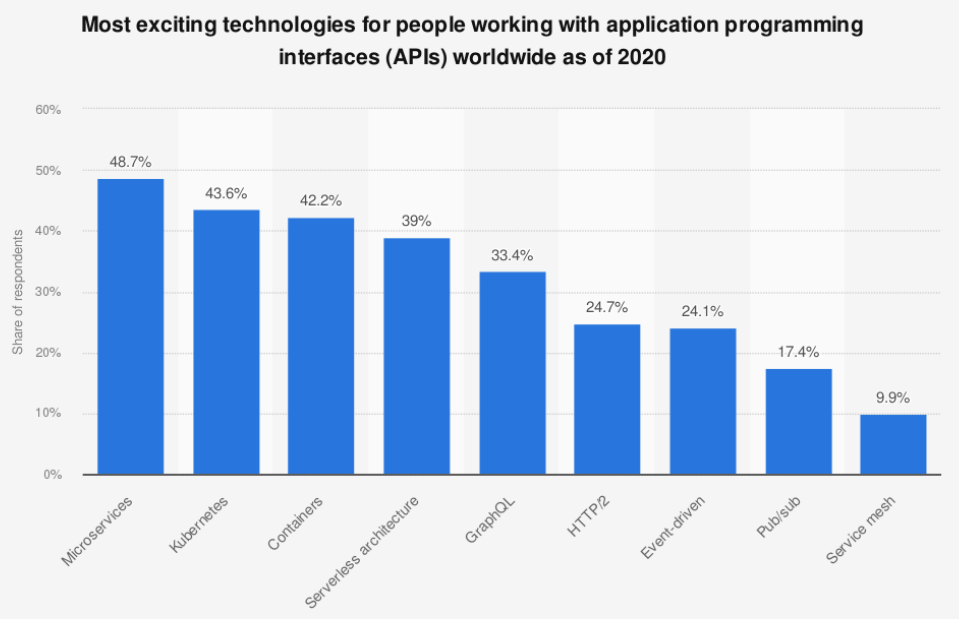
\includegraphics[width=1\textwidth]{img/appendix/StatistikMicroServices}}\\ % Pfad
		\source{\cite[][]{Statista2020a}} % Quelle
		\label{fig:StatistikMicroServices}
	\end{minipage}
\end{figure}

\begin{figure}[hbt!]
	\centering
	\begin{minipage}[t]{0.6\textwidth}	
		\caption{Konkrete Solutionarchitektur Beispielapplikation}
		\frame{\includegraphics[width=1\textwidth,page=3]{img/Beispielapplikation_Diagramm}}\\ % Pfad
		\source{Eigene Darstellung} % Quelle
		\label{fig:SolutionarchitekturBeispielapplikationKonkret}
	\end{minipage}
\end{figure}

\newpage
\begin{figure}[hbt!]
	\centering
	\begin{minipage}[t]{0.7\textwidth}	
		\caption{Vergleichbares Microfrontend für Evaluierung}
		\frame{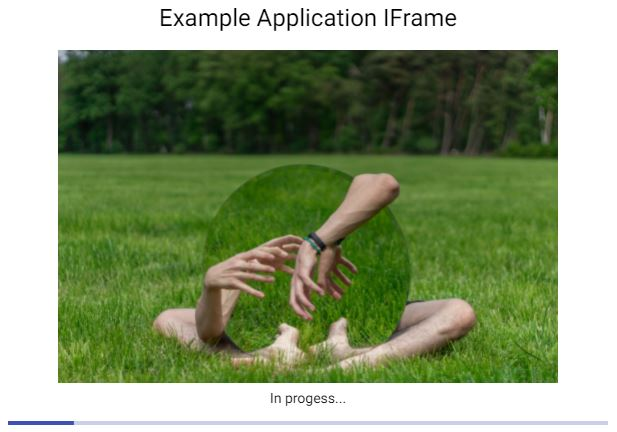
\includegraphics[width=1\textwidth]{img/appendix/Evaluierung_DarstellungBspApp}}\\ % Pfad
		\source{Eigene Darstellung} % Quelle
		\label{fig:EvalAnsicht}
	\end{minipage}
\end{figure}

\begin{figure}[hbt!]
	\centering
	\begin{minipage}[t]{1\textwidth}	
		\caption{Evaluierung Messung Iframe}
		\frame{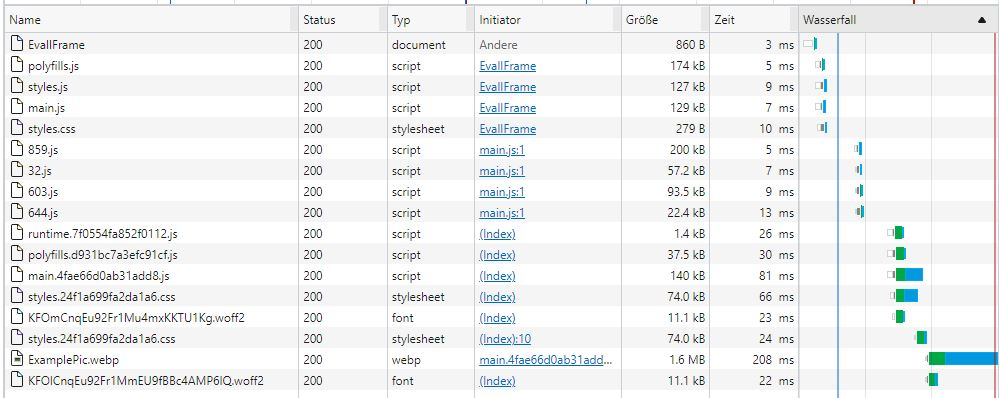
\includegraphics[width=1\textwidth]{img/appendix/Messung_IFrame}}\\ % Pfad
		\source{Eigene Darstellung} % Quelle
		\label{fig:MessungIFrame}
	\end{minipage}
\end{figure}

\newpage
\begin{figure}[hbt!]
	\centering
	\begin{minipage}[t]{1\textwidth}	
		\caption{Evaluierung Messung Web Component}
		\frame{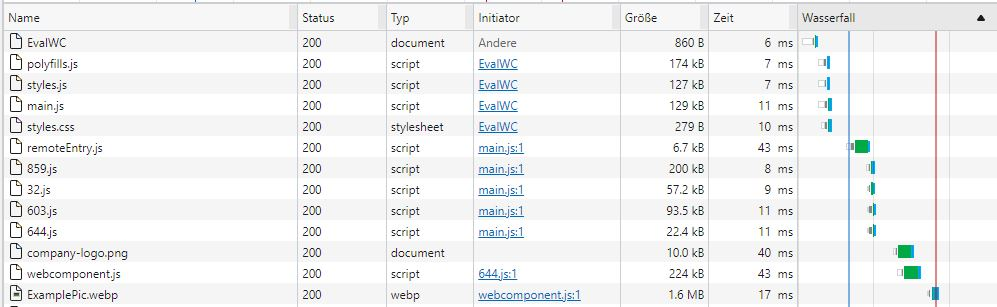
\includegraphics[width=1\textwidth]{img/appendix/Messung_WC}}\\ % Pfad
		\source{Eigene Darstellung} % Quelle
		\label{fig:MessungWebComponent}
	\end{minipage}
\end{figure}

\begin{figure}[hbt!]
	\centering
	\begin{minipage}[t]{1\textwidth}	
		\caption{Evaluierung Messung Module Federation}
		\frame{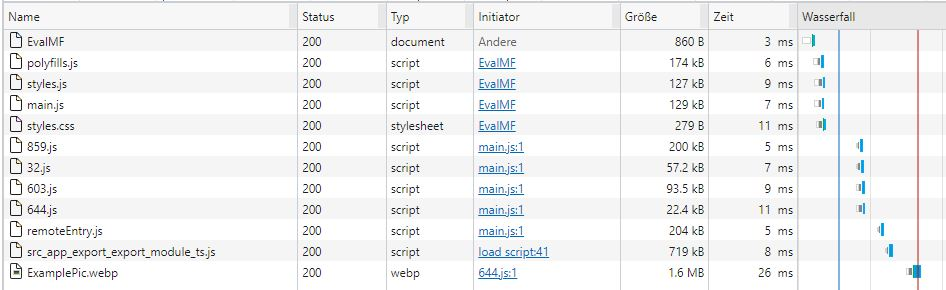
\includegraphics[width=1\textwidth]{img/appendix/Messung_MF}}\\ % Pfad
		\source{Eigene Darstellung} % Quelle
		\label{fig:MessungModuleFederation}
	\end{minipage}
\end{figure}

\begin{figure}[hbt!]
	\centering
	\begin{minipage}[t]{1\textwidth}	
		\caption{Evaluierung Messung Module Federation Web Components}
		\frame{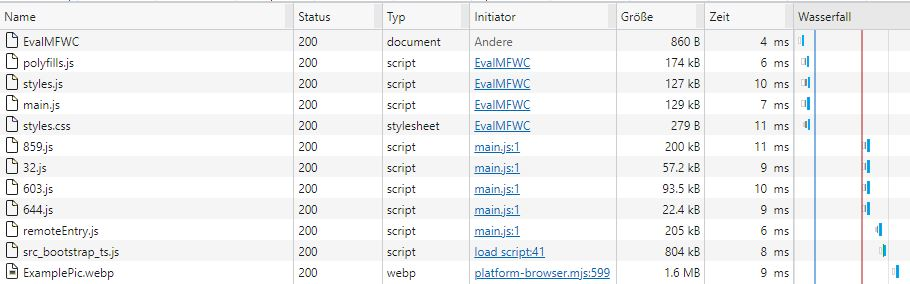
\includegraphics[width=1\textwidth]{img/appendix/Messung_MFWC}}\\ % Pfad
		\source{Eigene Darstellung} % Quelle
		\label{fig:MessungMFWC}
	\end{minipage}
\end{figure}

\newpage
\begin{figure}[hbt!]
	\centering
	\begin{minipage}[t]{0.65\textwidth}	
		\caption{HTML eines eingebundenen Iframes}
		\frame{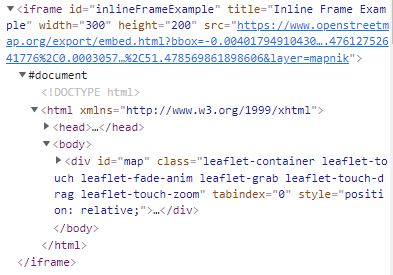
\includegraphics[width=1\textwidth]{img/appendix/IFrameHTML.JPG}}\\ % Pfad
		\source{Eigene Darstellung} % Quelle
		\label{fig:IFrameHTML}
	\end{minipage}
\end{figure}

\begin{figure}[hbt!]
	\centering
	\begin{minipage}[t]{0.6\textwidth}	
		\caption{Populärste Web Frameworks 2021}
		\frame{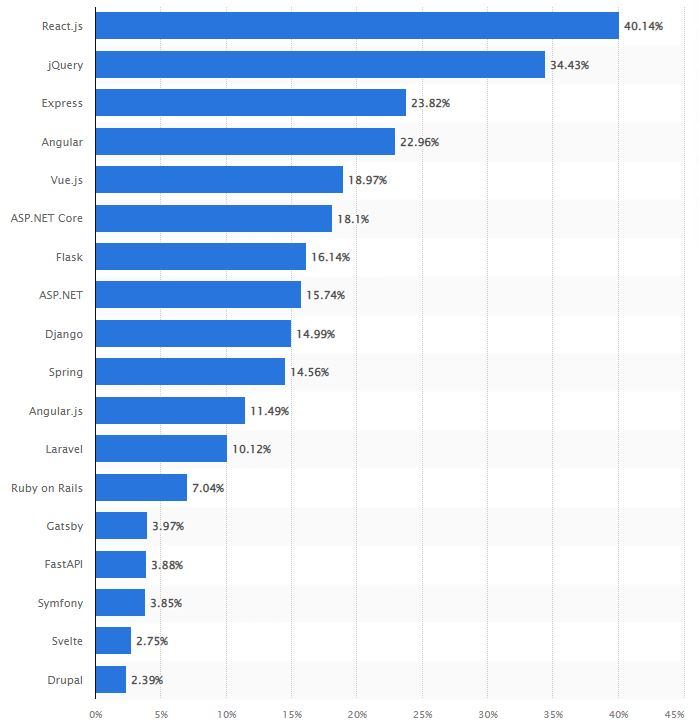
\includegraphics[width=1\textwidth]{img/appendix/FrontendFrammeworks.JPG}}\\ % Pfad
		\source{\cite[][]{Statista2022b}} % Quelle
		\label{fig:WebFrameworks}
	\end{minipage}
\end{figure}

\newpage
\begin{figure}[hbt!]
	\centering
	\begin{minipage}[t]{0.8\textwidth}	
		\caption{Marktanteile der führenden Browser}
		\frame{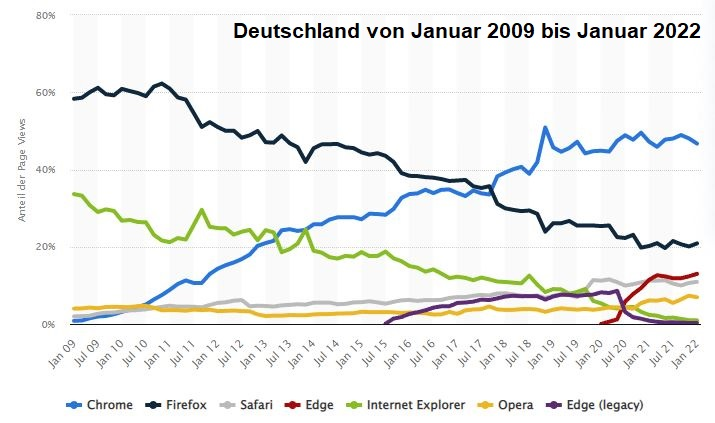
\includegraphics[width=1\textwidth]{img/appendix/StatistikBrowsernutzung.JPG}}\\ % Pfad
		\source{\cite[][]{Statista2022}} % Quelle
		\label{fig:StatistikBrowser}
	\end{minipage}
\end{figure}

\begin{figure}[hbt!]
	\centering
	\begin{minipage}[t]{0.8\textwidth}	
		\caption{Teilen von Daten bei Module Federation}
		\frame{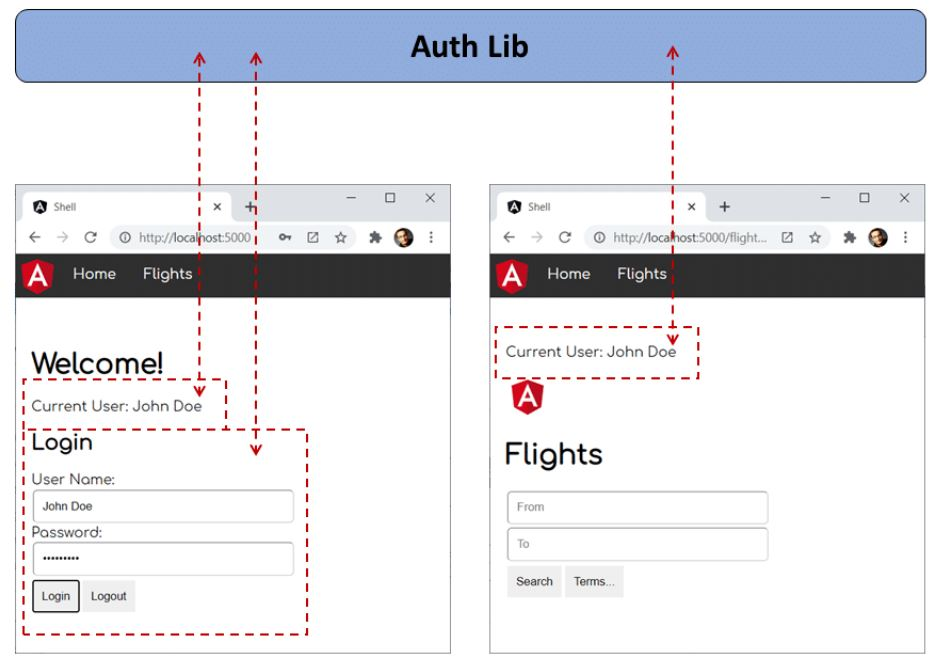
\includegraphics[width=1\textwidth]{img/appendix/ModuleFederationSharingData.JPG}}\\ % Pfad
		\source{\cite[][63]{Steyer2020}} % Quelle
		\label{fig:ModuleFShareData}
	\end{minipage}
\end{figure}

\newpage
\begin{figure}[hbt!]
	\centering
	\begin{minipage}[t]{1\textwidth}	
		\caption{Durchgeführte Messungen mit durchschnittlicher Datenmenge}
		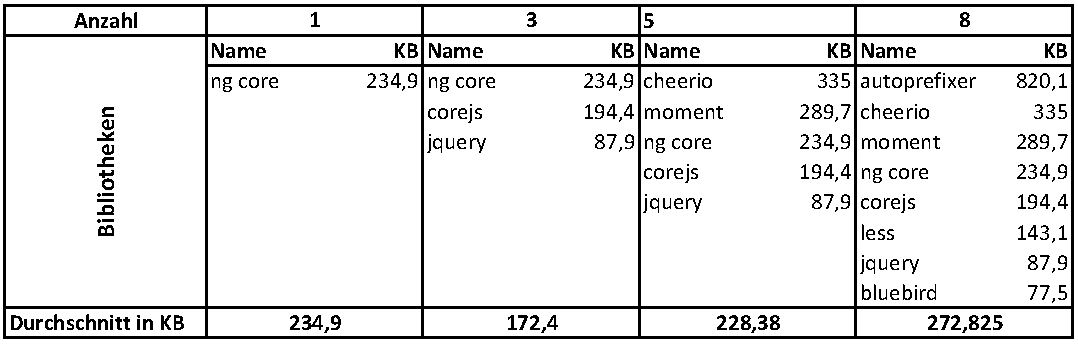
\includegraphics[width=1\textwidth]{img/appendix/DatasizeEval/GGBibliothekenMessungen.pdf}\\ % Pfad
		\source{Eigene Darstellung} % Quelle
		\label{fig:GGMessungBibs}
	\end{minipage}
\end{figure}

\begin{figure}[hbt!]
	\centering
	\begin{minipage}[t]{1\textwidth}	
		\caption{Doppelte Datenmenge durch zweifach eingebundenes Iframe}
		\frame{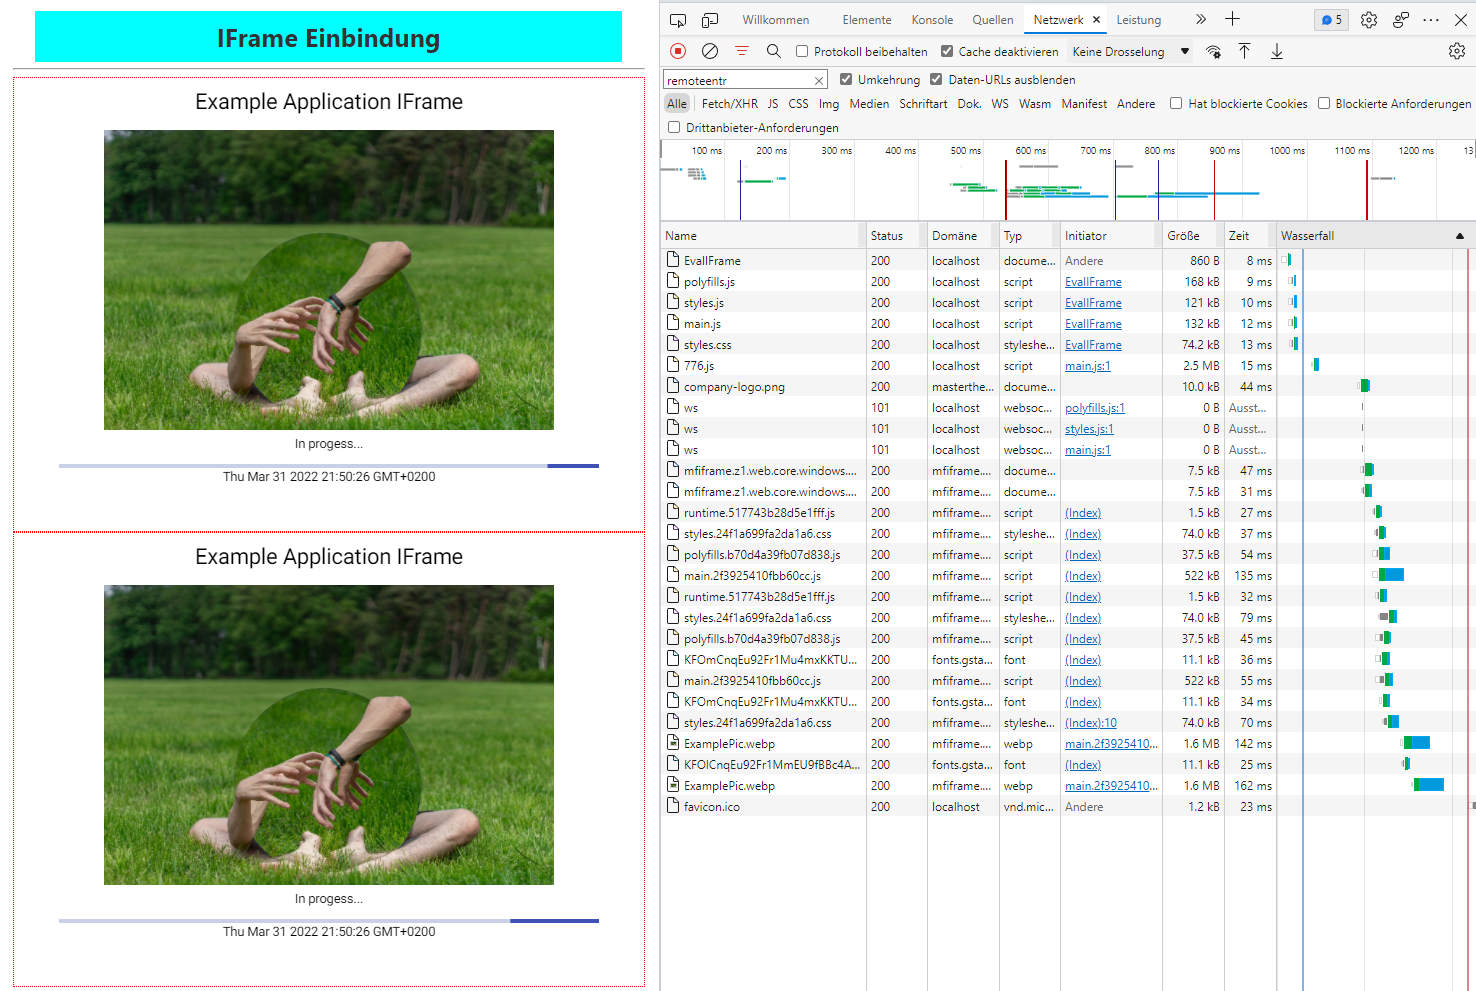
\includegraphics[width=1\textwidth]{img/appendix/Eval_Iframe_Skalierung}}\\ % Pfad
		\source{Eigene Darstellung} % Quelle
		\label{fig:EvalIframeSkalierbarkeit}
	\end{minipage}
\end{figure}

\newpage
\begin{figure}[hbt!]
	\centering
	\begin{minipage}[t]{0.5\textwidth}	
		\caption{Eingebundenes Iframe mit abgekapselten Stylings}
		\frame{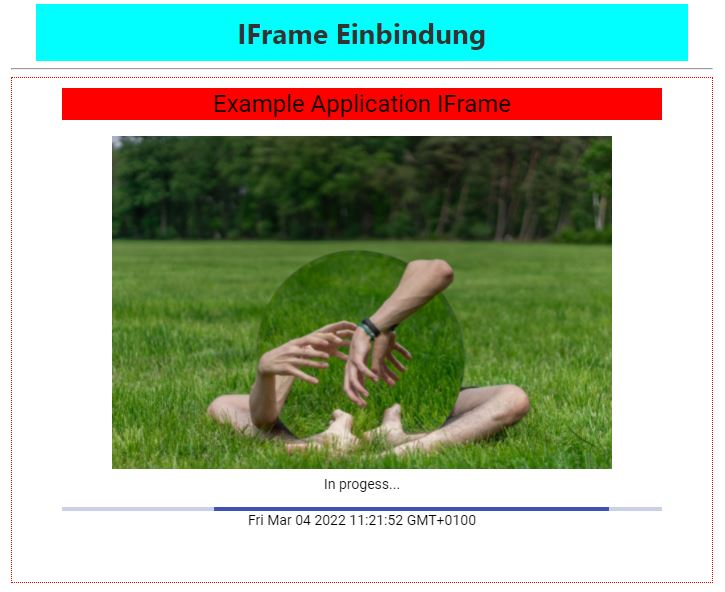
\includegraphics[width=1\textwidth]{img/appendix/Eval_Iframe_Beeinflussung.JPG}}\\ % Pfad
		\source{Eigene Darstellung} % Quelle
		\label{fig:EvalIframeBeeinflussung}
	\end{minipage}
\end{figure}

\begin{figure}[hbt!]
	\centering
	\begin{minipage}[t]{0.75\textwidth}	
		\caption{Sequenzdiagramm einer Zusammensetzung durch Nginx SSI}
		\frame{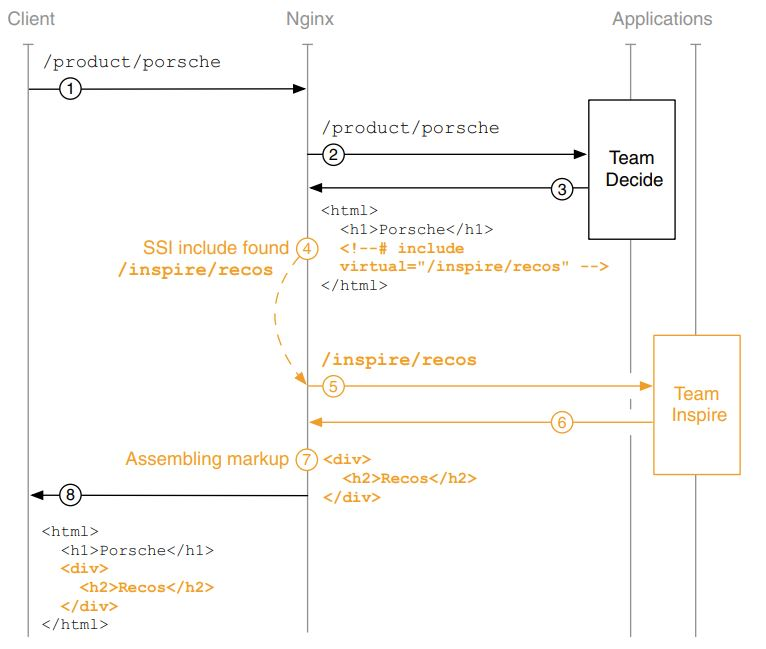
\includegraphics[width=1\textwidth]{img/appendix/SSCNginxSSI}}\\ % Pfad
		\source{\cite[][62]{Geers2020}} % Quelle
		\label{fig:SSCNginxSSI}
	\end{minipage}
\end{figure}

\newpage
\begin{figure}[hbt!]
	\centering
	\begin{minipage}[t]{1\textwidth}	
		\caption{Entscheidungsbaum Technologie Microfrontends}
		\frame{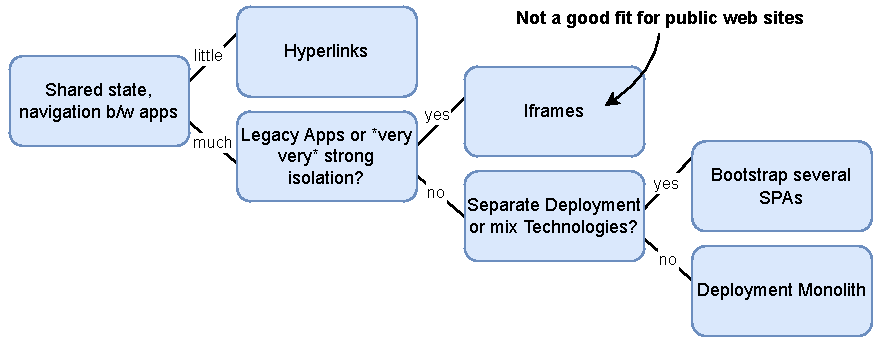
\includegraphics[width=1\textwidth]{img/appendix/EntscheidungsbaumArchitekturMF}}\\ % Pfad
		\source{\cite[Eigene Darstellung in Anlehnung an][]{Steyer2018}} % Quelle
		\label{fig:EntscheidungsbaumArchitekturMF}
	\end{minipage}
\end{figure}

\begin{figure}[hbt!]
	\centering
	\begin{minipage}[t]{0.7\textwidth}	
		\caption{Laden der Wetter Web Component}
		\frame{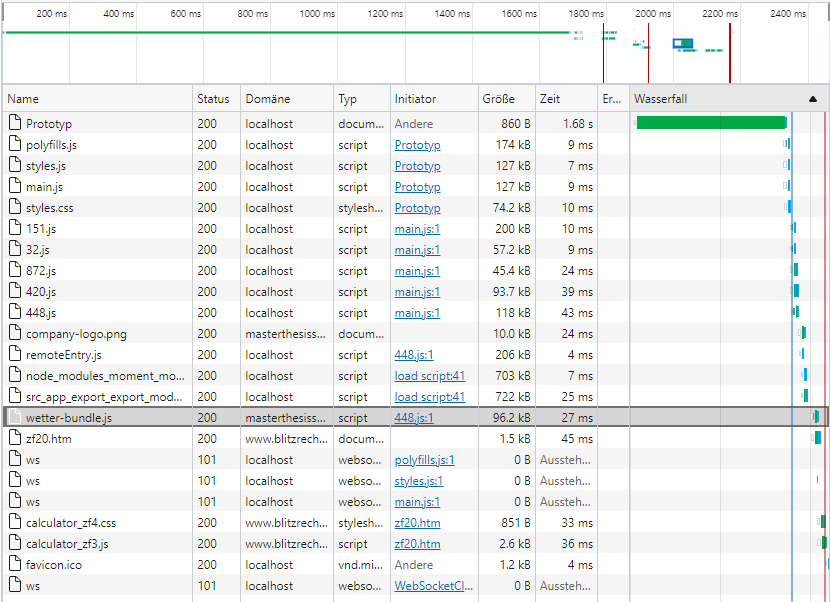
\includegraphics[width=1\textwidth]{img/appendix/PrototypEinmaligesLadenWC}}\\ % Pfad
		\source{Eigene Darstellung} % Quelle
		\label{fig:PrototypEinmaligesLadenWC}
	\end{minipage}
\end{figure}

\newpage
\begin{figure}[hbt!]
	\centering
	\begin{minipage}[t]{0.6\textwidth}	
		\caption{Event Emitter zum Übertragen von Daten}
		\frame{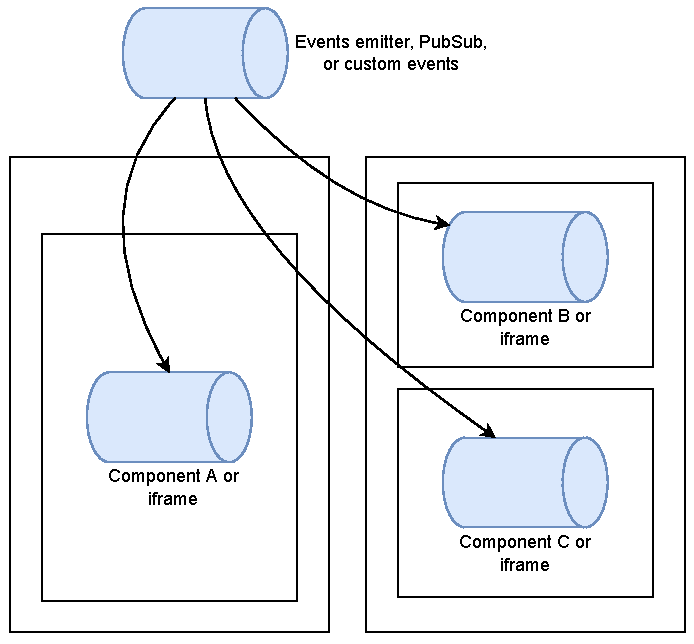
\includegraphics[width=1\textwidth]{img/appendix/MFSharingDataEventEmitter}}\\ % Pfad
		\source{\cite[Eigene Darstellung in Anlehnung an][33]{Mezzalira2021}} % Quelle
		\label{fig:MFSharingDataEventEmitter}
	\end{minipage}
\end{figure}

\begin{figure}[hbt!]
	\centering
	\begin{minipage}[t]{0.55\textwidth}	
		\caption{Web Storage zum Teilen von Daten}
		\frame{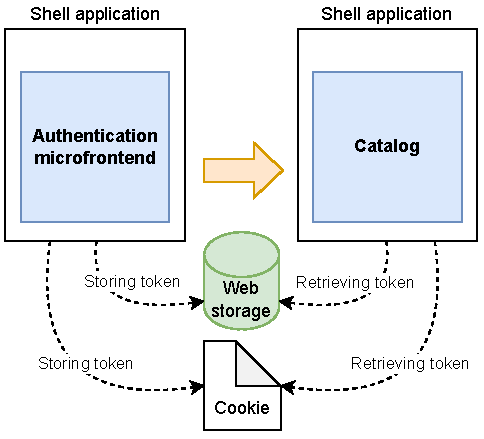
\includegraphics[width=1\textwidth]{img/appendix/MFSharingDataWebStorage}}\\ % Pfad
		\source{\cite[Eigene Darstellung in Anlehnung an][34]{Mezzalira2021}} % Quelle
		\label{fig:MFSharingDataWebStorage}
	\end{minipage}
\end{figure}

\newpage
\begin{figure}[hbt!]
	\centering
	\begin{minipage}[t]{0.65\textwidth}	
		\caption{Beispielhafte realisierte Lokalisierung bei Amazon}
		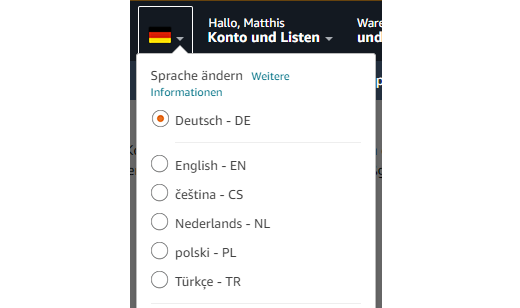
\includegraphics[width=1\textwidth]{img/appendix/PortalshellLokalisierung.PNG}\\ % Pfad
		\source{Screenshot von Amazon} % Quelle
		\label{fig:PortalshellLokalisierung}
	\end{minipage}
\end{figure}

\begin{figure}[hbt!]
	\centering
	\begin{minipage}[t]{0.65\textwidth}	
		\caption{Zusammengefasste Präferenzmatrix mehrerer Teilnehmer}
		\includegraphics[width=1\textwidth]{img/Präferenzmatrix}\\ % Pfad
		\source{\cite[Eigene Darstellung in Anlehnung an][194]{Schierenbeck2016}} % Quelle
		\label{fig:PraeferenzmatrixBefuellt}
	\end{minipage}
\end{figure}

\newpage
\begin{figure}[hbt!]
	\centering
	\begin{minipage}[t]{0.65\textwidth}	
		\caption{Web Component in der eigenen Anwendung eingebunden}
		\frame{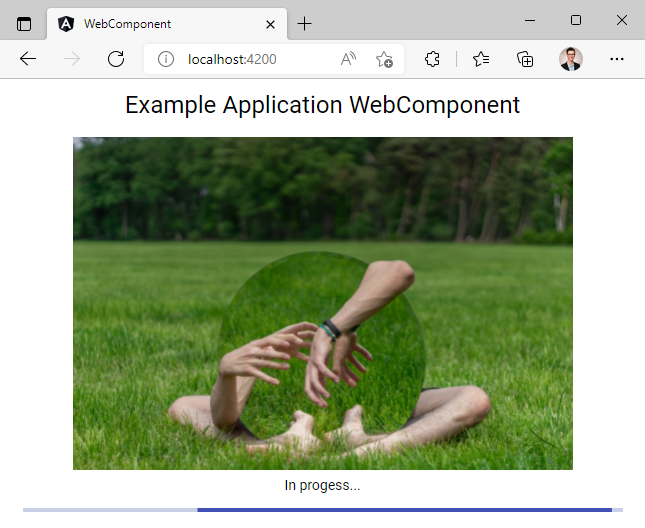
\includegraphics[width=1\textwidth]{img/appendix/WCSelbstEinbindung}}\\ % Pfad
		\source{Eigene Darstellung} % Quelle
		\label{fig:WCSelbstEinbindung}
	\end{minipage}
\end{figure}

\begin{figure}[hbt!]
	\centering
	\begin{minipage}[t]{0.65\textwidth}	
		\caption{Module Federation WC Beeinflussung Styles}
		\frame{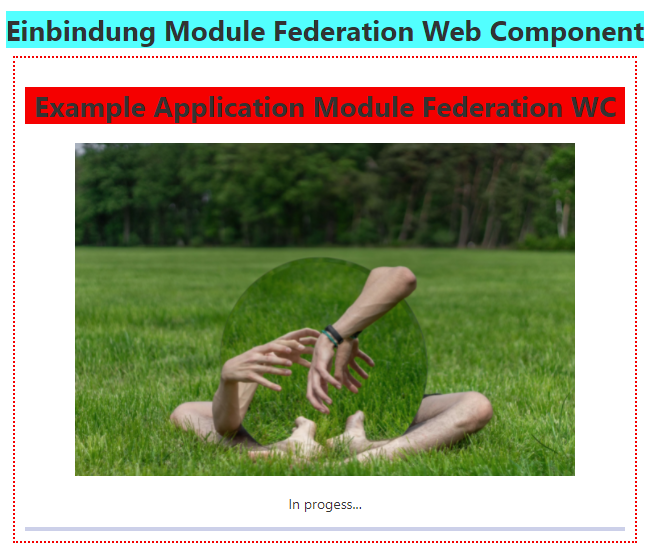
\includegraphics[width=1\textwidth]{img/appendix/Eval_MFWC_Beeinflussung.PNG}}\\ % Pfad
		\source{Eigene Darstellung} % Quelle
		\label{fig:EvalMFWCBeeinflussungStyles}
	\end{minipage}
\end{figure}

\newpage
\begin{figure}[hbt!]
	\centering
	\begin{minipage}[t]{0.65\textwidth}	
		\caption{Ladezeiten Module Federation WC bei 8 geteilten Bibliotheken}
		\frame{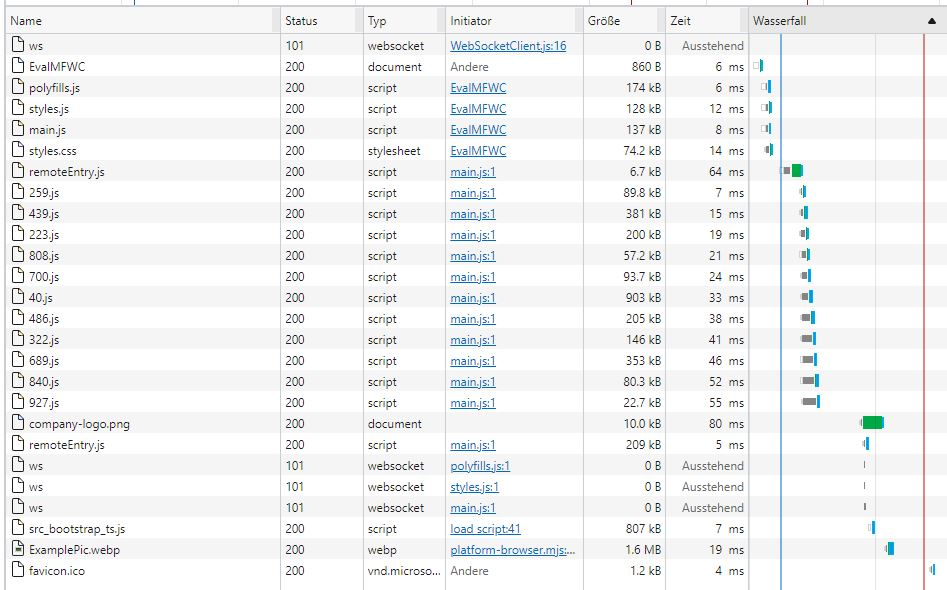
\includegraphics[width=1\textwidth]{img/appendix/DatasizeEval/MFWC_8.JPG}}\\ % Pfad
		\source{Eigene Darstellung} % Quelle
		\label{fig:EvalMFWCLadezeit}
	\end{minipage}
\end{figure}

\begin{figure}[hbt!]
	\centering
	\begin{minipage}[t]{0.7\textwidth}	
		\caption{Horizontaler Wissensaustausch in vertikalen Teams}
		\frame{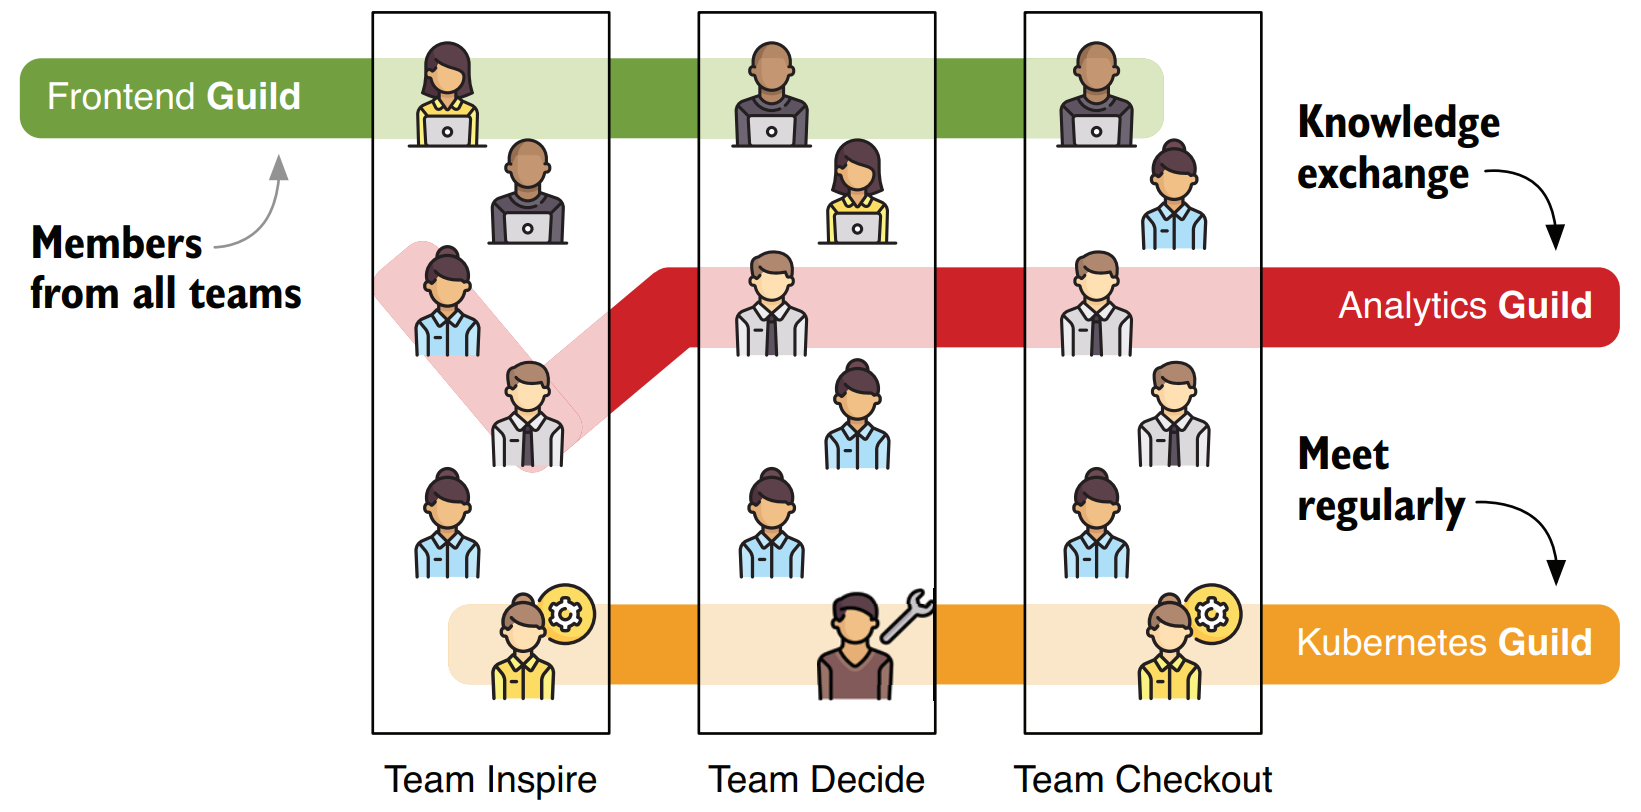
\includegraphics[width=1\textwidth]{img/appendix/VertikaleTeamsWissensaustausch.PNG}}\\ % Pfad
		\source{\cite[][244]{Geers2020}} % Quelle
		\label{fig:VertikaleTeamsWissensaustausch}
	\end{minipage}
\end{figure}

\newpage
\begin{figure}[hbt!]
	\centering
	\begin{minipage}[t]{0.75\textwidth}	
		\caption{Schnittmengen von Frameworks bei Module Federation}
		\frame{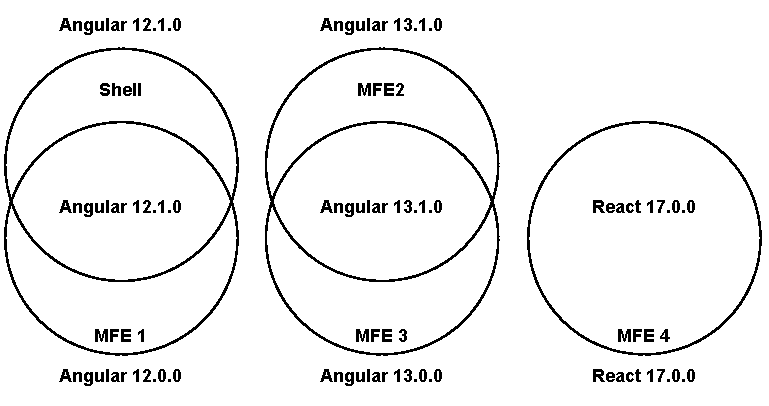
\includegraphics[width=1\textwidth]{img/appendix/ModuleFederationWebComponentsDifferentFrameworkVersions}}\\ % Pfad
		\source{\cite[Eigene Darstellung in Anlehnung an][]{Steyer2021a}} % Quelle
		\label{fig:ModuleFederationSchnittmengenFrameworks}
	\end{minipage}
\end{figure}

\begin{figure}[hbt!]
	\centering
	\begin{minipage}[t]{0.65\textwidth}	
		\caption{Monolithisches Frontend vs. Microfrontend}
		\frame{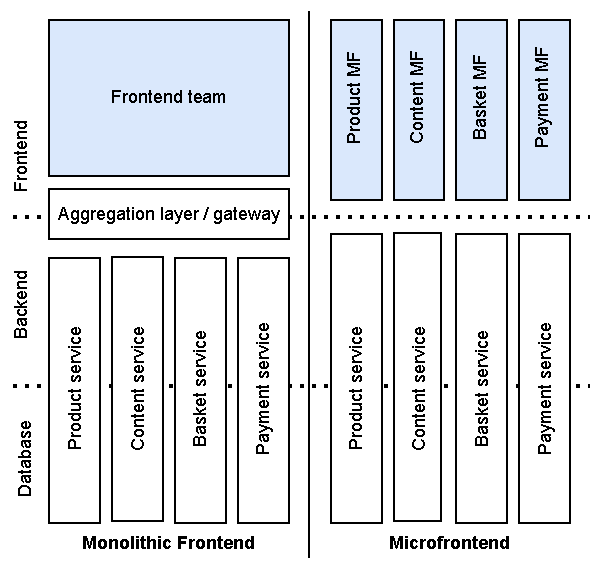
\includegraphics[width=1\textwidth]{img/appendix/MonolithicMicrofrontend}}\\ % Pfad
		\source{Eigene Darstellung} % Quelle
		\label{fig:MonolithicMicrofrontend}
	\end{minipage}
\end{figure}

\newpage
\begin{figure}[hbt!]
	\centering
	\begin{minipage}[t]{1\textwidth}	
		\caption{Skalierung Web Component doppelte Einbindung}
		\frame{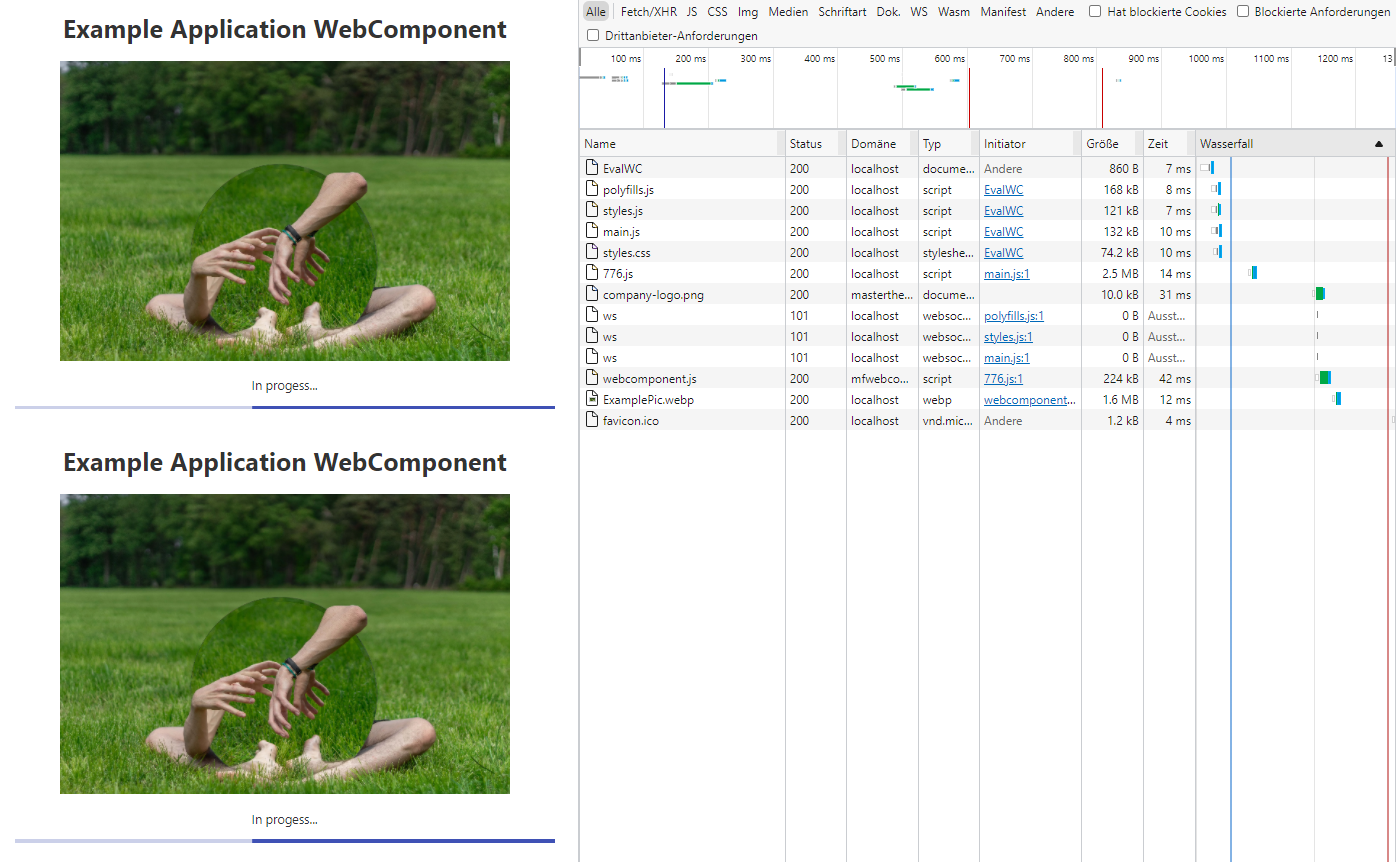
\includegraphics[width=1\textwidth]{img/appendix/Eval_WC_Skalierbarkeit}}\\ % Pfad
		\source{Eigene Darstellung} % Quelle
		\label{fig:EvalWCSkalierbarkeit}
	\end{minipage}
\end{figure}

\begin{figure}[hbt!]
	\centering
	\begin{minipage}[t]{1\textwidth}	
		\caption{Histogramm der Datenmenge von NPM-Paketen}
		\frame{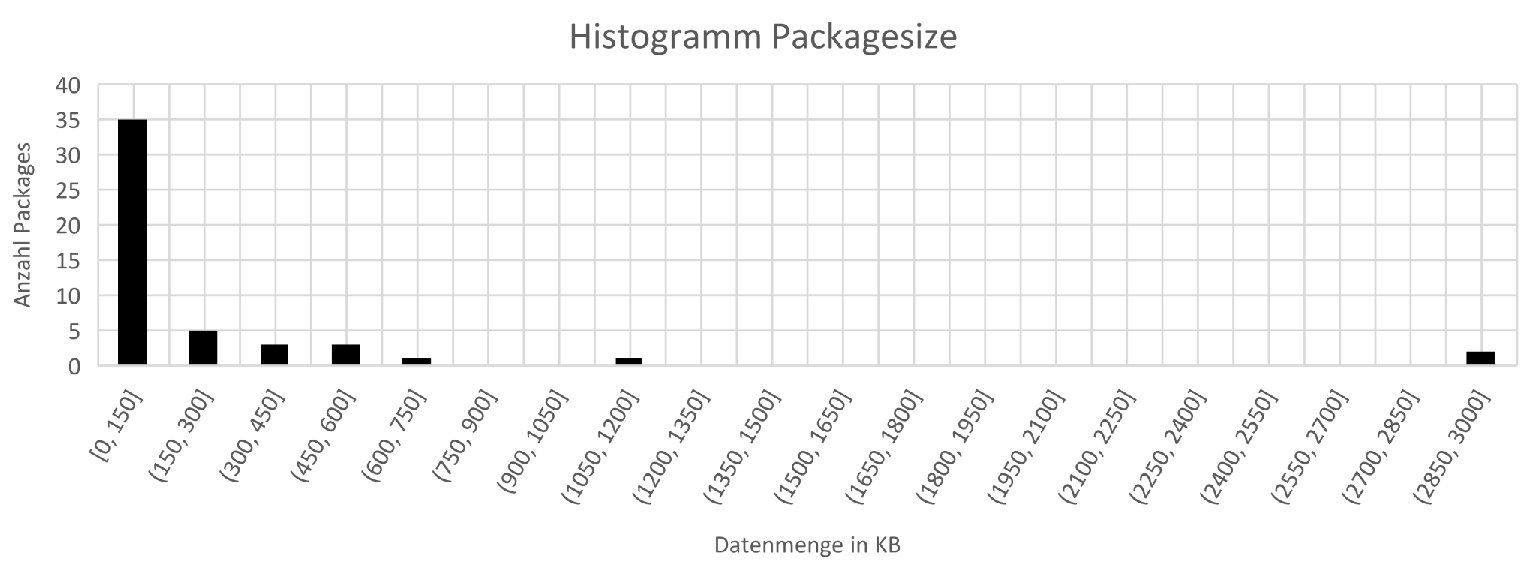
\includegraphics[width=1\textwidth]{img/appendix/DatasizeEval/Histogramm}}\\ % Pfad
		\source{Eigene Darstellung} % Quelle
		\label{fig:HistogrammDatenmenge}
	\end{minipage}
\end{figure}

\newpage
\begin{figure}[hbt!]
	\centering
	\begin{minipage}[t]{1\textwidth}	
		\caption{Übersicht der Elemente der Portalapplikation mit Beispielen}
		\frame{\includegraphics[width=1\textwidth,page=5]{img/Beispielapplikation_Diagramm}}\\ % Pfad
		\source{Eigene Darstellung} % Quelle
		\label{fig:PortalapplikationElementeKonkret}
	\end{minipage}
\end{figure}

\begin{figure}[hbt!]
	\centering
	\begin{minipage}[t]{1\textwidth}	
		\caption{Laborsetup der Messungen}
		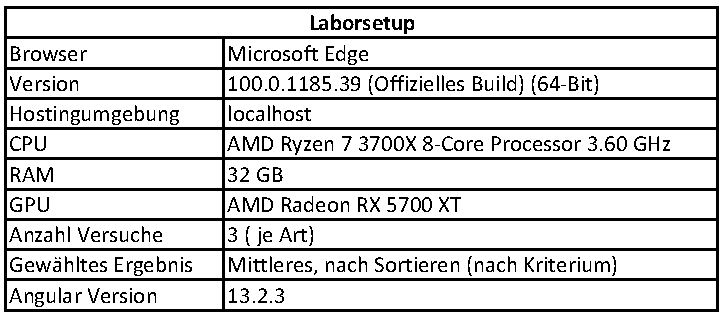
\includegraphics[width=1\textwidth]{img/appendix/Laborsetup}\\ % Pfad
		\source{Eigene Darstellung} % Quelle
		\label{fig:Laborsetup}
	\end{minipage}
\end{figure}

\newpage
\begin{figure}[hbt!]
	\centering
	\begin{minipage}[t]{0.7\textwidth}	
		\caption{Funktionsweise einer Portalapplikation}
		\frame{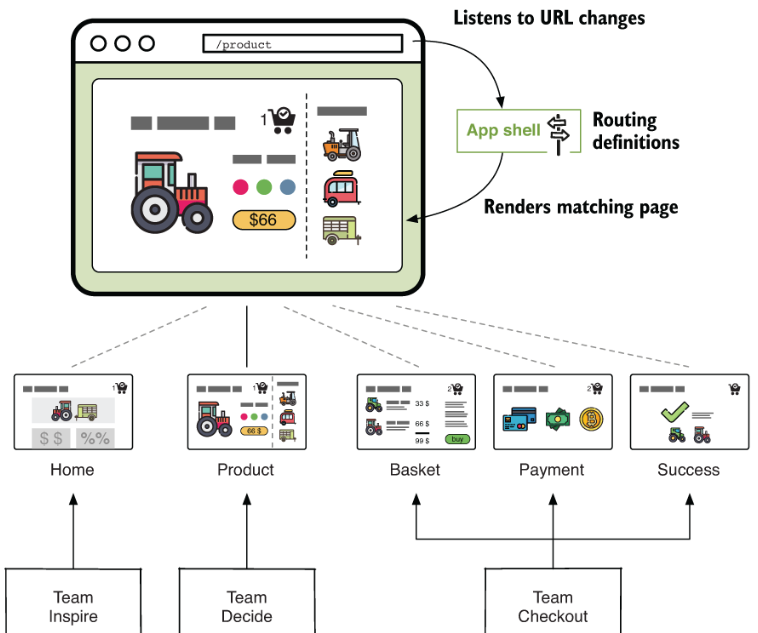
\includegraphics[width=1\textwidth]{img/appendix/AufgabenShell}}\\ % Pfad
		\source{\cite[][121]{Geers2020}} % Quelle
		\label{fig:AufgabenShell}
	\end{minipage}
\end{figure}

\begin{figure}[hbt!]
	\centering
	\begin{minipage}[t]{1\textwidth}	
		\caption{Microfrontend mit \textit{moment.js} geteilt durch Module Federation}
		\frame{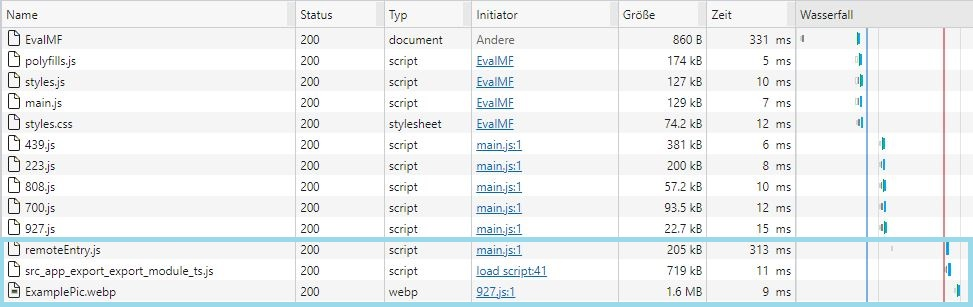
\includegraphics[width=1\textwidth]{img/appendix/Messung_Moment_MF_Shared}}\\ % Pfad
		\source{Eigene Darstellung} % Quelle
		\label{fig:MomentMF}
	\end{minipage}
\end{figure}

\newpage
\anhang{Tabellen}\label{app:Tabellen}

\begin{table}[!hbt]
	\centering
	\begin{minipage}[t]{1\textwidth}
		\caption{Verwendete NPM-Pakete zum Vergleich der Datenmenge} % Überschrift
		\begin{tabularx}{\columnwidth}{| X | X |}
			\toprule
			\thead{\textbf{Name}} & \thead{\textbf{Datenmenge in KB (Stand 28.02.2022)}}\\
			\midrule
			autoprefixer & 820.1 \\
			cheerio & 335  \\
			moment & 289.7 \\
			@angular/core & 234,9 \\
			corejs & 194.4 \\
			less & 143.1 \\
			jquery & 87.9 \\
			bluebird & 77.5 \\			
			\midrule
			Durchschnitt & 272.8 \\
			\bottomrule
		\end{tabularx}
		\source{Eigene Darstellung}
		\label{tab:BibliothekenDatenmenge}
	\end{minipage}
\end{table}

\begin{table}[hbt]
	\centering
	\begin{minipage}[t]{\textwidth} % Breite, z.B. 1\textwidth		
		\caption{Übersicht der Rollen der prototypischen Portalshell} % Überschrift
		\begin{tabularx}{\columnwidth}{|c|c|X|}
			\toprule
			ID & Rollenname 		& Beschreibung \\
			\midrule
			1 & Anwender 				& Der Anwender darf die Portalapplikation benutzen, aber nichts konfigurieren. Er sieht die Dashboards seines Mandanten und kann die Microfrontendinstanzen in den Dashboards benutzen.\\
			\midrule
			2 & Administrator 			& Der Administrator darf die Portalapplikation sowie die Microfrontendinstanzen vollumfänglich nutzen. Er kann neue Benutzer registrieren und ihnen Rollen zuweisen. Ebenfalls sieht der Administrator eventuell mehr Inhalte in den Microfrontendinstanzen, sollte es dort Bereiche geben, die ausschließlich für Administratoren zugänglich sind. Der Administrator ist ebenfalls in der Lage Microfrontendinstanzen auf einem Dashboard zu platzieren und neu anzuordnen.\\
			\bottomrule
		\end{tabularx}
		\source{Eigene Darstellung}
		\label{tab:RollenPortalapplikation}
	\end{minipage}
\end{table}

\newpage
\anhang{Expertengespräche}\label{app:Expertengespräche}
\deffeat{Exp1}\\ \\
\underline{Expertengespräch mit Hanno Kortekamp}

Gesprächsprotokoll mit Hanno Kortekamp, Senior Software-Architekt bei einem großen deutschen IT-Dienstleister, mit mehr als 10 Jahren Berufserfahrung in Entwicklung und Betrieb von Portalapplikationen.\\
Durchgeführt am 20.12.2021 zu den Themen: Microfrontends, Portalapplikationen und Module Federation.

\textbf{Querschnittsaspekte von Portalapplikationen} 
\begin{compactitem}
   \item SDK für Formularelemente, Theme, UI und Styleguide
   \item Authentifizierung und Autorisierung
   \item Konfiguration
   \item Lokalisierung
   \item Navigation
   \item Mandantenfähigkeit
\end{compactitem}

\textbf{Messkriterien für Integration Microfrontends} 
\begin{compactitem}
	\item Übertragene Datenmenge
	\item Renderingzeit bis Darstellung
	\item Entwicklungsaufwand / Wartbarkeit
	\item Nähe am Standard
	\item Unterstützung verschiedener Frameworks
	\item (Browser)Kompatibilität
	\item Autonomie
	\item Unabhängigkeit der Entwicklerteams
	\item Lock-In Effekt	
\end{compactitem}

\textbf{Einsatz Module Federation im Projekt} 
\begin{compactitem}
	\item Nur Module Federation beschränkt Unabhängigkeit der Entwicklerteams
	\item Web Components in Kombination mit Module Federation mehr flexibel
\end{compactitem}

\newpage
\deffeat{Exp2}\\ \\
\underline{Expertengespräch im Rahmen der Nutzwertanalyse}

Diskussion im Rahmen der Nutzwertanalyse. Teilnehmerkreis bestehend aus:\\
Zwei Software-Architekten, zwei Software-Entwicklern und einem IT-Projektmanager.\\
Alle Teilnehmer haben bereits mehrjährige Erfahrungen mit Portalapplikationen und Microfrontends sammeln können.

Durchgeführt am 03.02.2022 zu den Themen: Vorstellung \& Diskussion gesammelter Kriterien sowie anschließende individuelle Durchführung der Paarvergleichsmethode. 

\textbf{Gesammelte Kriterien:}
\begin{compactitem}
	\item Datenmenge
	\item Renderingzeit
	\item Entwicklungsaufwand
	\item Wartbarkeit
	\item Nähe zum Standard
	\item Frameworks
	\item Kompatibilität
	\item Autonomie
	\item Unabhängige Entwicklerteams
	\item Lock-In Effekt
\end{compactitem}

Sowie Ergänzung des Kriteriums \textit{Interoperabilität}.

Anschließend individuelle Durchführung der Paarvergleichsmethode. Die einzelnen Paarvergleichsmatrixen sind dem beigefügten Anhang \ref{app:SonstigeDokumente} enthalten und in der \textit{Paarvergleichsmatrixen.zip} zu finden.

\newpage
\anhang{Sonstige Dokumente}\label{app:SonstigeDokumente}
Hinweis: Die sonstigen Dokumente sind nur in der beigefügten zip-Datei enthalten.\\

\begin{compactenum}
	\item Internetquellen
	\item Tabelle Nutzwertanalyse
	\item Tabellen Paarvergleichsmatrixen
	\item Tabelle Berechnung übertragene Datenmenge
	\item Messergebnisse geteilte Bibliotheken Web Components
	\item Quellcode Microfrontends
	\item Quellcode Portalshell inkl. StatistikApp
\end{compactenum}